%ihi_aunas@yahoo.com
\documentclass{article}
\usepackage{graphicx} % Required for inserting images
\usepackage{mmacells}
\usepackage{float}

\usepackage{dialogue}
\usepackage{tikz}
\usepackage{natbib}
\usepackage{setspace}
\usepackage{tabularx}

\usepackage{amsmath}
\usepackage{amsthm}
\usepackage{amssymb}

\newtheorem{theorem}{Theorem}
\newtheorem{proposition}[theorem]{Proposition}
\newtheorem{lemma}[theorem]{Lemma}
\newtheorem{definition}[theorem]{Definition}

\begin{document}
\title{A Task-Based View of Generative AI}
\author{John Horton\\MIT \& NBER}
\date{\today{}}

\newcommand{\machine}[1]{\langle #1 \rangle}
\newcommand{\human}[1]{( #1 )}
\newcommand{\cost}[1]{C\{ #1 \}}

\maketitle

\begin{abstract}
\noindent The distinctive feature of generative AI is that it generates: code, writing, images, music, videos, and so on, and does so at essentially zero marginal creation cost.
These generations are made in response to some request or ``prompt.''
But these AI generations only become economic goods if judged suitable for some human need.
This depends on human judgment in the evaluation, the skill in crafting the prompt, and the technical capability of the generative model. 
When deciding to route a task to an  AI, the question is whether the prompt-evaluation loop inherent in using that AI will be more efficient than simply doing the task by hand. 
Tasks can be efficiently changed together, in the sense that each task feeds into the next without human intervention.
A task might be added to an automated chain even, if the human has an absolute advantage in that task in isolation.
\end{abstract}

\onehalfspacing

\section{Introduction}
Economic models on the effects of technology have to make simplifying assumptions about what that technology does and cannot do.
The ``problem'' with generative AI, from an economic modeling standpoint, is that is unclear what AI \emph{cannot} do even now, never mind over the next 5 or 10 years. 
As such, it seems prudent to move away from what they cannot do and instead try to identify what is likely to be a constant, no matter how much capabilities advance.

No matter how capable these models become, three human tasks remain:
1) deciding to ask the AI to do some task, 
2) asking the AI to do that task, and 
3) evaluating the machine's efforts. 
Each of these steps is a human-provided task that can, in turn, be AI-augmented. 

I present a model of tasks previously done by humans instead of being completed in concert with humans. 
The decision to route to an AI depends not only on the theoretical capabilities of the AI for a task, but how well the AI is likely to do, given the prompting and judgment of the human operator. 
This is meta-knowledge about a combined AI-human system.

\paragraph{Generative AI generates ``stuff'' in response to human requests, but that stuff is not necessarily an economic good.}
The distinctive feature of generative AI is that it generates: writing, code, images, music, videos, and so on.
What the AI generates is not simply a random draw of things the AI could produce.
Rather, it produces something in response to some human request or ``prompt.''
What AI generates is not inherently useful. 
The raw output must be evaluated and deemed suitable through judgment.
This assessment can then influence where the human asks the AI to modify the output in the required direction. 
This creates a human-AI hybrid loop of prompting and judging. 
And upstream of all of this is the necessary human insight into routing, or whether the task is one that an AI is likely to lead to a good outcome, with the prompting and evaluation the worker can provide. 

\paragraph{Whether a machine can ``do'' a task is an economic question, not a technical question.}
The task could be ``answer questions about the text in a document'' and whether an AI can do this task depends on the payoff to doing it correctly. 
The firm might be fine letting a machine do low-level customer service support; we might be very hesitant to let it handle queries from major institutional investors.

\paragraph{Generative AI is an information goods factory, but it has human workers.}
Generative AI is that it works with us to produce information goods. 
And the economic-so-what is that the machines can do their part of the productive process at zero marginal cost---or at least at a cost that will likely trend to zero.

Digitization already pushed the marginal reproduction costs and distribution costs for information goods to zero---but the costs of initially producing those goods remained high: I could costlessly share an ebook with you, but writing a book was still a long, hard slog.

\paragraph{Tasks have a recursive structure}
Every task can be divided into smaller sub-tasks, creating a recursive structure.
For a human, we think of anyone as being able to do a task as also being able to do every constituent sub-task.
A machine might only be able to do some sub-set of those tasks. 

And what constitutes a ``task'' is likely to move to higher and higher levels of abstraction: 
From ``find typos in this ad copy'' to ``create ad copy'' to ``create a marketing campaign, launch, execute and monitor performance'' to ``increase sales'' to ``run the business profitably'' to $\ldots$.  

\paragraph{The logic of comparative advantage and communication costs tend to create serial dependencies between tasks within jobs, creating an o-ring-like production structure}
In the model, tasks within a job have serial dependencies. 
There are economic forces that push this characterization to be true. 
If a job lacked serial dependencies between tasks, we could likely reap more gains for specialization.
It costs us too much to hand off a task.
We only do it when we cannot do the task or the labor savings are so great it is worth it. 
The labor savings are great when management costs are low: the task is easy to describe, easy to evaluate, and has a high probability of success. 

\paragraph{Using an AI for some task has qualitative similarities to delegating a task to another human or team.}
The decision to use an AI bears similarities to the decision to delegate some task to a subordinate.
And conditional upon delegation, the skill of using AI bears similarities to the management of people and teams. 
Deciding whether the output is sufficient requires judgment, whether the output is human-produced or otherwise. 

\paragraph{Goods differ in their cost of human evaluation, which changes the cost of using AI for production.}
The extent of generative AI usage depends on the costs of judging the model's output.
This cost could vary considerably based on the nature of the good.
An analogy is drawn to the process by which consumers evaluate goods. 
Search goods are trivially easy to evaluate (and hence ideal candidates for AI creation), whereas inspection goods and credence goods might have prohibitively expensive evaluation costs. 
These differences will affect the adoption of AI by task.

\paragraph{Entrepreneurial innovation will focusing reducing AI management tasks as well as increasing model abilities}
We will see investment to improve the capabilities of models but also try to reduce the costs of prompting and to reduce the cost of the evaluation. 
The skills that AI complements are themselves potential targets for AI assistance. 
We will likely see AIs that help write prompts or make it easier for humans to express themselves.  
We will see AIs and related technologies that help evaluate output. 

\paragraph{AI will create new labor-labor substitution possibilities for ``Rick Rubin'' reasons.}
In light of the change in what is delegated, I discuss how labor-labor substitution might change who performs a task. 
In particular, job redesign will take advantage of the fact that skills in judging output are separate from the skill of creating some output.
There are food critics who cannot cook; record producers who cannot play instruments; technologists who cannot program, and so on.
As AI makes it so that humans no longer have to do every task in a job, AI might open up jobs to people who are otherwise blocked by a skill they lack.
However, that task has to be marginal (assuming other blocking tasks are not also automated). 
For example, identifying a bone fracture in an X-ray does not mean a person is ready to be a radiologist.
I.e., if there was only one task that precluded them from doing some occupation, then AI might allow them to do that occupation.
Allowing more people to do more tasks could have an indirect productivity effect. 
Ironically, the harder the task to perform, the more potential for AI to unlock this substitution potential, as the pool of potential prompters and judges is much larger than the pool of doers.

\paragraph{Generative AI can produce predictions but also other information goods.}
The literature to date has emphasized AI as a prediction technology \citep{agrawal2019}. 
Although this is an area where they can sell, this seems, with hindsight, to be too narrow of a framing.
Generative AI models have shown the ability to create output similar to or better than even expert humans can produce over a broad class of knowledge-processing tasks.  
Consistent with this view, experimental evidence at knowledge worker tasks shows large productivity gains using ChatGPT for a collection of knowledge worker tasks \citep{noy2023experimental}.
%A machine that can return flawless Python, javascript, and HTML in response to a prompt that says ``build me a web app that can do X, Y, and Z" is not making predictions.
%Drafting a memo for me about some topic, generating music that millions enjoy, analyzing a data set, and making plots---also not predictions. 

A prediction is an information good. 
But it is also an experience good that might reveal its quality over a long time frame, depending on the nature of the prediction. 
Once you know a prediction is good; it is probably useless other than as a data point that you should value the predictions of the machine more.
If it is a prediction about what might happen, but that could be changed given the firm's actions, it could be a credence good.
This is precisely the kind of task that the relative benefit of using an AI might be quite low if the ability to judge is low. 

\paragraph{Generative AI substitutes ``maker labor'' and complements ``manager labor'' in the short-run.}
In the model, there are just two broad ``kinds'' of labor: 
Labor that does tasks, and labor that manages an AI doing that task. 
While we might think there is some correlation between the cost of the machine and the human doing the task, this seems like an imprudent assumption.

We should not presume that tasks that are hard for humans are easy for computers or vice versa. 
We do hard, time-consuming tasks because the output is valued. 
Playing excellent chess \emph{seemed} like the kind of thing computers can do well. 
Generating photorealistic art, playing diplomacy, and generating new programs on the fly did not seem like tasks where computers would show capabilities.

All else equal, more capable management increases the number of tasks an AI performs, holding AI capabilities fixed. 

\paragraph{A automation chain is when constituent tasks are chained together without a human requesting an output or evaluating that output.}

\paragraph{A ``job'' will disappear when every constituent task is subsumed by an automation chain.}
Jobs can disappear when all the tasks in the sequence can be chained without human oversight between tasks. 

\paragraph{The cost properties of adjacent tasks in the chain influence the chained automation decision.}
Being adjacent to a highly automatable task will tend to ``pull'' that task into an automated chain.

\paragraph{The economic returns to improving an AI's capabilities depend on human cost for that task.}
The AI has to be good enough that the human management of the AI becomes worthwhile. 
Language models have existed for years.
One could have tried to use it for any number of tasks. 

\paragraph{More capable models will require more expressive domain-specific languages, making ``asking'' a highly skilled task}
%The set of possible things an AI can return has to  
%Imagine I ask an AI to do some task.
%There is a set of all possible responses that AI could make, $R$.
%Let the index of that task be $i$.
%Let $A_i$ be the ``acceptable'' answers that could be returned. 
$q_i = Pr\{R(i) \in A_i\}$

%We might think of the space of all things that could be returned in response to some prompt, a subset of which is %``acceptable.'' 
$q = Pr(a \subset A)$.
%If every point in $A$ is reachable with a prompt, the expressiveness of the prompt language has to be as large as the space of answers. 
%What is the pre-image of $A$?

%A new domain-specific language for asking a machine to create information goods.
%This new language is far closer to English. 
%It will not remain primarily written but will, over time, be multi-modal.
%The limit becomes how well you can express what you want, 

\paragraph{Useful simplifications in the characterizations of technology}

For example, \cite{autor2003skill}'s ``computation substitutes for routine cognitive tasks and complements non-routine cognitive tasks'' is a useful simplification of what computers do. 
Or technology automates some tasks previously done by humans but also spurs new tasks which only humans can do, at least for some time \citep{acemoglu2019}. 
Or AI is a prediction technology that lowers prediction costs, increasing the value added by labor that complements prediction. 

\paragraph{What we know about the labor market task capabilities of generative AI suggest they can do many tasks well.}
The rise of generative AI has challenged the plausibility of older simplifications.
The fraction of tasks currently performed by workers in the US that might be done or augmented with LLMs is considerable \citep{eloundou2023gpts}.
The other problem is that these new technologies have not yet had their economic impact, so our historical data can tell us little about how technology is likely to affect the economy. 

\paragraph{Jobs with few tasks are more prone to full automation}

\paragraph{Jobs where the next task is unpredictable are more resistant to full automation}

\section{Task-based view}

Imagine there are just two tasks, $q_1$ and $q_2$.
The possibilities are
\begin{enumerate}
 \item Both done by human: $(1)(2)$
 \item Both done by machine, but not chained: $<1><2>$
  \item Both done by machine and chained: $<1|2>$
  \item One by machine, 


\end{enumerate}

\subsection{Definition of a ``task''}
A natural question is the delineation of these tasks---where does one begin and the other end? 
Tasks can be subdivided, with every step capable of being broken into smaller steps.\footnote{
    Writing a memo has the subtask ``write the first line of the memo'' then ``write the second line of the memo.''
    ``Write the first line of the memo'' and can be broken into ``first word'' and ``first letter'' and ``keystroke down, then keystroke up.''    
}
For our purposes, a helpful delineation is some sequence of tasks such that an AI could, in principle, do that whole sequence of constituent sub-tasks.
The capabilities of the AI model make the tasks. 
The start of the task is the first point where some human direction about what to do is required. 

One might think that evaluation itself could be the domain of the AI, but if the model could have improved the chance the output would be evaluated positively, that process would have already been incorporated into the model. 
What is left is the residual evaluation that a human must uniquely supply: judgment.

If they choose to use an AI, the human asks the AI to perform the task with a prompt. 
The AI tries to perform the task, generating output.
The worker then evaluates the output to decide if it is suitable. 
If it is, the worker can continue to the next task 
If it is not, the human can try to modify the prompt and re-evaluate the new output until the need is satisfied. 

\section{A model of production}
Imagine a job as tasks to be performed in sequence $1, 2, \ldots n$.
Let $C_h$ be a vector of costs to a human for performing each task.
Let us consider a single task with a cost $c_{h}$.

In addition to having the human do the task, there is an AI that can do the task instantly at zero marginal cost, but it only succeeds with probability $q$, given the optimal effort by the human at ``prompting.''
Each prompt costs the human $c_p$, and each evaluation of an AI output costs the human $c_e$.
This constant $q$ is a simplification, as we might expect the ``first'' $q$ to be low for a given prompt, but then increase with each subsequent prompt that is a refinement.
Let $c_p + c_e = c_m$, with $m$ for management.
This $q$ captures the model's capability but also reflects the capability of the human at prompting and judging.
Figure~\ref{fig:flow} illustrates the situation.

\begin{figure}
\caption{A job with a task decomposed into sub-tasks} \label{fig:flow}
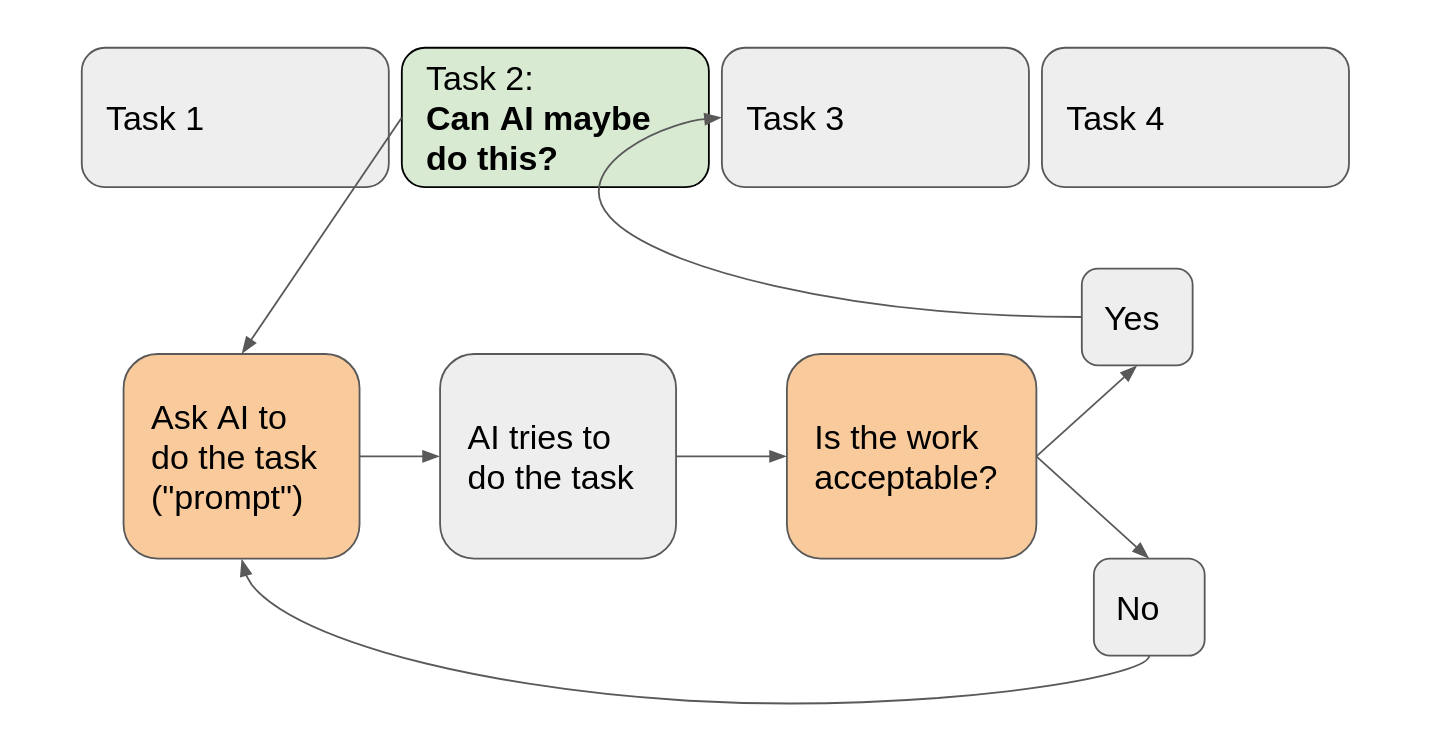
\includegraphics[width = \textwidth]{flow.png}
\end{figure}

We will use the notation $\human{\cdot}$ to indicate a task done by a human, $\machine{\cdot}$ as done by an AI.
As a mnemonic, the curved parenthesis captures the greater flexibility of humans. 

\begin{lemma}
 For a given task, it is cheaper to automate if $\cost{\machine{1}} < \cost{\human{1}}$, which happens when $c_m / q < c_h$.
\end{lemma}
\begin{proof}
The expected cost of using the AI is $c_m/q$ (recall ${\sum_{k=1}^\infty q^k (1-q)^{k-1} = 1/q}$) and so 
the task will be automated if
    \begin{align}
    q > \frac{c_m}{c_h}. \nonumber
\end{align}
\end{proof}

This decision criterion has some intuitive comparative statistics.
The higher the human performance costs, the more likely a worker is to try an AI, even a fairly incapable one (i.e., low $q$).
The lower the prompting and evaluation costs, the more likely an AI will be used.
If we think of novice workers as having higher own-performance costs, or high $c_h$ values, they might be more likely to use an AI.

It seems likely, empirically, that prompting costs are sub-linear with respect to $c_h$.
The prompt ``write me a haiku about economics'' is about the same effort as ``write me an epic poem about economics'' but the $c_h$ differs radically. 
To the extent $c_h$ and $c_e$ vary less than $c_h$, we should expect a size bias, with more attempts to use for larger tasks in the $c_h$ sense.  

\subsection{Chaining together tasks}
AI tasks can be chained together, creating a new task with a success probability equal to the product of all the constituent tasks.
The chained-together task still has human prompting and evaluation at the start and end.
Notation-wise, a $|$ indicates chained-together tasks, e.g.,  $\machine{1|2}$ indicates a machine does tasks 1 and 2.
The $|$ is meant to evoke the *nix pipe.
Only AI tasks are capable of being chained.

Consider an $n = 5$ job. 
If $\machine{1|2}\human{3}\human{4}\machine{5}$, it would indicate tasks 1 and 2 done in a chain by a machine.  
The per-pass success probability of $\machine{1|2}$ is $q_1q_2$. 
Tasks 3 and 4 would be done by humans, while task 5 would be done by an AI. 
Total costs for the good would be $\frac{c_m}{q_1 q_2} + c_{h(3)} + c_{h(4)} + \frac{c_m}{q_5}$.

Note that with an $n$ task jobs, there are $2^{n-1}$ possible task partitions.
Each singleton can be done by a human or a machine; each sequence is done only by a machine.
Later, I will discuss algorithmic approaches for finding the cost-minimizing allocation of tasks to humans and machines.

\begin{definition}
Let $T^*$ be the cost-minimizing combination of humans and computers for some sequence of tasks.
\end{definition}

\subsection{When to chain two tasks both done by machine}
The decision to chain two automated tasks is simple: chain if $q_1 + q_2 > 1$.
This is given in Lemma~\ref{lemma:chain}.

\begin{lemma} \label{lemma:chain}
If $q_1 + q_2 > 1$, then $\cost{\machine{1|2}} < \cost{\machine{1}\machine{2}}$.  
\end{lemma}
\begin{proof}
One possibility is that we put them together; another is to split them apart and have a human manager at each step.
If we chunk the task, costs are $\frac{c_m}{q_1q_2}$, whereas if we split them up, we have $\frac{c_m}{q_1} + \frac{c_m}{q_2}$.
We chunk to tasks if 
\begin{align}
\frac{1}{q_1 q_2} <\frac{1}{q_1} + \frac{1}{q_2}
\end{align}
which is true when $q_2 + q_1 > 1$, otherwise they should be split. 
\end{proof}

\begin{lemma}
A $T^*$ cannot have a chained machine sequence with sum of $q$ values less than 1.
\end{lemma}
\begin{proof}
Suppose we have a chain in $T^*$ with $Q = q_1 q_2\ldots q_k$.
WLOG, take the smallest $q$ in the chain, $q_\epsilon$.
\begin{align}
 \frac{1}{q_{\epsilon}} + \frac{1}{Q/q_{\epsilon}} < \frac{1}{Q}\\
 \frac{Q/q_{\epsilon}}{Q} + \frac{q_{\epsilon}}{Q} < \frac{1}{Q}\\
 Q/q_{\epsilon} + q_{\epsilon} < 1 \\
 Q + q_\epsilon^2 < q_{\epsilon}
\end{align}

\end{proof}

\subsection{Cost minimization problem: shortest path through a tree}
The cost minimization each $A$ node splits into three possibilities: a) have a human do the task, b) have a machine do the task, but do not chain it with the previous task, (c) add another task and chain it. 
Figure\ref{fig:tree} illustrates the tree. 
The cost minimization problem is to find the shortest path through the tree. 

We can prune the tree by removing all nodes where $\human{i}$ is in the label, but $\cost{\human{i}} > \cost{\machine{i}}$ and the AI-equivalent, i.e., $\machine{i}$ is in the label but $\cost{\human{i}} < \cost{\machine{i}}$.
We can also prune all nodes where there is a machine sequence $\machine{K}$ and $\sum_{k \in K} q_k < 1$ because such a node can be split up.

\begin{figure}
\caption{The possible production scenarios with an $n=2$ task job}
\label{fig:tree}
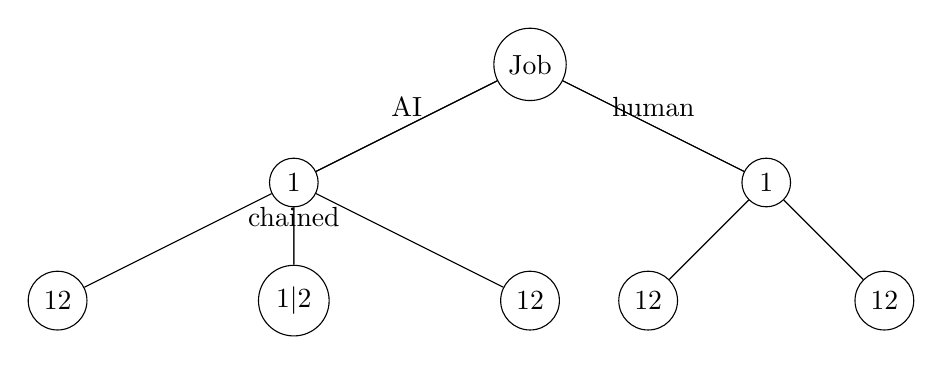
\begin{tikzpicture}[
  level/.style={sibling distance=60mm/#1}
]
\node[circle, draw] (S) at (0,0) {Job}
  child {node[circle, draw] (A) {$\machine{1}$}
    child {node[circle, draw] (AA) {$\machine{1}\machine{2}$}}
    child {node[circle, draw] (AAC) {$\machine{1|2}$}} 
    child {node[circle, draw] (AH) {$\machine{1}\human{2}$}} 
  }
  child {node[circle, draw] (H) {$\human{1}$}
    child {node[circle, draw] (HA) {$\human{1}\machine{2}$}}
    child {node[circle, draw] (HH) {$\human{1}\human{2}$}}
  };
\path (S) edge node[midway, above] {AI} (A);
\path (S) edge node[midway, above] {human} (H);
\path (A) edge node[midway, above] {chained} (AAC);
\end{tikzpicture}
\end{figure}

When $n = 1$, there are just two child nodes, one human, one AI: $H_1 = 1$, $A = 1$.
With $A_{n+1} = 3 A_{n}$ and $H_n = 2 H_n$

\paragraph{If you should chunk a task, it should be with the relatively more reliable process}

\begin{lemma} \label{lemma:pair_better}
 If a task can be combined with either a more or less reliable chain, if it should be combined, it should be combined with the lower-cost chain.
 If $\cost{\machine{1}} > \cost{\machine{3}}$, then $\cost{\machine{1}\machine{2|3}} < \cost{\machine{1|2}\machine{3}}$.
 \end{lemma}
\begin{proof}
Suppose you have $q_L$, $q$, and $q_H$, in sequence, with $q_H > q_L$.
Assuming you will chunk left or right, which chunk to you choose?
\begin{align}
 \frac{1}{q_L} + \frac{1}{q q_H} < \frac{1}{q_L q} + \frac{1}{q_H} \\
  q q_H + q_L < q_H + q q_L \\
  q (q_H  - q_L) < q_H - q_L.
\end{align}
\end{proof}

In light of \ref{lemma:pair_better}, if we use a divide-and-conquer algorithm, we need ``repair'' edges when we combine tasks.
For example, suppose we have an optimal sub-sequence, $T_L$ and $T_R$ that we want to combine.
If the end of $T_L$ is $\machine{k|k+1}$ and the start of $T_R$ is $\machine{k+2}$, it might be the case that the new sequence if $\machine{k}\machine{k+1|k+2}$. 
It might trigger a cascade of changes that make divide-and-conquer infeasible.

\subsection{A task might be automated even if humans have a comparative advantage in doing that task because of chaining possibilities}
\begin{lemma}
A task might be automated even if humans have a comparative advantage over machines in doing that task:
$C\{\human{1}\machine{2}\} < C\{\machine{1}\machine{2}\}$ does not imply $C\{\human{1}\machine{2}\} < C\{\machine{1|2}\}$.
\end{lemma}
\begin{proof}
We can see this with a counterexample.
The machine success probabilities are $q_1 = 3/5$ and $q_2 = 4/5$.
Management costs are the same for both tasks, $c_m = 1$.
Human performance costs for the first task is $c_h = 3/2$.
Let the human performance cost for the second task be $\infty$, so it must be automated. 
Note that for the first task, it is cheaper to have the human do it: 
$c_h < c_m / q_1$, as the human cost is just $3/2 = 9/6$ but the AI cost is $5/3 = 10/6$.
However, we fully automate the costs are 
$c_m / (q_1 q_2) = 25/12$. 
If we do the first by hand and automate the second, we have total costs of $c_h + c_m / q_2 = 11/4$, or $33/12$.
Thus, even though humans have a comparative advantage in a task, we might chain it with another task and manage the combined task.
\end{proof}

\subsection{Improvements in model capabilities increase the viability of productive chains}

\paragraph{More capable AIs substitute for doer labor; have mixed effects on management labor}
Raising $q$ had three effects on human labor. 
It displaces direct doing labor, as it is more likely that $(c_h + c_e)/q < c_h$, but increases the demand for management-labor of the extensive margin, as more tasks flip from being done by a human to being done by a machine.
Raising $q$ also causes more tasks to be chained, which also economizes on management labor---if it did not, there would be no reason to switch.
It also decreases the demand for management on intensive margin by lowering $C/q$.

A job exists if all those tasks where it is more economical for the user to do the task themselves than assign it to someone else.
Assigning a task to someone else requires (a) asking them to do it, for $c_p$

\subsection{Algorithmic solution to optimal machine/human collaboration}
You have a collection of tasks, $T$, indexed by $i$.
At the start, assume each is done by a human i.e., $T_0 = \human{1}\human{2}\human{3}\ldots \human{n}$.
Let $C\{T\}$ be the cost of some allocation of machines and humans to a sequence of tasks, $T$.
\begin{enumerate}
\item For each task in $T$, decide if it should be done by a machine, even without any ``chaining.'' 
$C\{\machine{i}\} \le C\{\human{i}\}$.
Ignoring subscripts, this is just $c_{h} < c_{m} / q$.
\item Find $i$ with the largest value of $q_i + q_{i + 1}$ in $T_j$.
\item For that $i$, if $C\{\machine{i | i + 1}\}$ is the smaller than costs of of $\machine{i}\machine{i + 1}$, $\machine{i}\human{i+1}$, $\human{i}\machine{i + 1}$, ``chunk'' tasks $i$ and $i+1$. This means replace the $i$th position in $T$ with a new automated task with $q_{i'} = q_i q_{i+1}$. Delete the $i + 1$ position task.
\item Go back to step 2 and repeat. If $T_{j + 1} = T_{j}$, i.e., there are no more substitutions to produce, stop.
\end{enumerate}

\begin{theorem}
 Combining tasks greedily with respect to cost reductions yields $T^*$.
\end{theorem}
\begin{proof}
 Greedy always stays ahead? Brute force a bunch of these to make sure algorithm works. Also, allow flexibility in $c_m$ too. 
\end{proof}


\subsection{What does ``full automation'' mean?}
Full automation consists of finding places in the production process where the costs of replacing the asking and evaluation steps with an AI are economical because the quality is sufficiently good and the cost of an evaluation failure is relatively low. 
For example, consider the task ``respond to customer inquiry'' previously done with a human representative. 
That human might take an inquiry and respond, perhaps with templates matching certain common questions and links to so-called knowledge-base articles. 
But even with a fairly rudimentary chatbot limited to a response of the form ``given your question, here are some resources you might find useful'' to replace this aspect of the customer service task.
The ``ask the AI to do something'' has been offloaded to the customer, as has the evaluation step is left to the consumer.
This full automation is just externalizing the prompting and evaluation costs to consumers, which presumably has some negative effect on demand.  

If the AI is doing the prompting and evaluation, we can think of $c_e$ and $c_p$ as de facto zero.
The failure mode is then the one step in the chain passes a bad prompt to the next. 
If the prompt and evaluation step has a very high $q$, this concern is not so great. 
Why do we not have an evaluation step? 
The prompt for the next task in the chain is the output from the previous step: there is no new effort, and this is already optimized to do that task as well as it can. 
There is also no distinct evaluation step. Why? 
Because if the AI could improve $q$ by evaluation on its own, that would already be included in the process it uses. 
The overall chain of unreliable components gives a $q = q_1 \cdot q_2 \cdot q_3$.
We can then consider just the human sandwich of prompting and evaluation, with this sequence of tasks in the middle.  

With a more advanced AI, it might try to answer a question directly.
This is common now. 
But it is unlikely that the task ``respond to current institutional investor inquiry'' would be turned over to even a sophisticated AI given the risks.

The modeling primitives are similar to \cite{kremer1993}.
With a chain of tasks, the value of improving one link is proportional to the product of all the other links.
No effort is valuable if there is a $q = 0$ link.
Suppose performance improvements all have the same marginal cost. 
A multiplicative process implies focusing efforts on the weakest link or the smallest $q'$, as this. 
In that case, the marginal return is $(\prod_k q_k)/q'$, which by definition, offers the largest return.



\subsection{Product market (speculative)}
A potential product, $k$ is defined by a vector of success probabilities $Q$, human production costs, $C_H$; management costs $C_M$   $(Q, C_H, v)$ and an associated product market value $v$.

Managerial labor and production labor is supplied to the market competitively.
A product is produced in equilibrium if $v \ge \cost{T_{Q,C_H,C_M}^*}$.
The price is production costs. 
Let $D_k(\cdot)$ be the demand curve for $k$.
The $S_k(w_h, w_m, Q)$ is the number of jobs producing that output, which could be zero if not cost-competitive.

\begin{proposition}
Lowering costs of any kind does not reduce the number of viable products.
\end{proposition}

\begin{definition}
An improvement in AI is when there exists a $j$ such that $Q'_i > Q_i$ and for all other indices $j$, $Q'_j \ge Q_j$
\end{definition}

\begin{proposition}
An improvement in AI capabilities does not increase costs: ${\cost{T^*_{Q'}} \le \cost{T^*_{Q}}}$.
\end{proposition}
% NB: There is some assumption to be made about distribution of tasks and costs such that costs decrease


\subsection{AI usage as a managerial skill}
The routing, prompting, and evaluation tasks are similar to a manager's tasks.
Generative AI seems to complement a new kind of managerial skill, albeit the management of an AI. 
But given humans are harder to change the machines, it seems likely that AIs will continue to be modified to make it so that humans can manage them. 

Knowing what to yourself versus delegating, giving good instructions conditional upon delegating, and evaluating output---and course-correcting as necessary--- is closely similar to simply managing people.
Being a judge of talent, scoping and explaining projects in ways people will understand, giving good, actionable feedback, and so on. 
It is not fundamentally different from what should be delegated to a human. 

Adding ``let's think step by step'' to a prompt can dramatically increase performance \citep{kojima2023large}.

If instead of the AI producing the good costlessly, then some delegated worker has to do it. 
Suppose their wage is $w_1$, and they will take $t_1$ units of time.
A ``boundary of the job'' definition where a worker does the tasks is those where the costs of delegating to a specialist are greater than the cost savings. 
The difference is that when delegating to a worker, the costs are non-zero.
I do a task myself when $w_{0} t_{0} < (c_p + c_e + w_{1} t_{1})/q$.
I might delegate a task when (a) the person is higher-paid but must be more efficient (low $t_{1}$), the costs of managing are low (low $c_p$ and $c_e$), or the person is not as efficient by lower wage, $w_{1} < w_{1}$.

\subsection{Returns to more capable models}
Investments that raise task success probability, $q$, have two effects. 
They lower costs inframarginal for all tasks that the AI was already used for, with the elasticity of total costs equal to negative 1 in $q$, i.e., a 10\% increase in $q$ lowers expected AI costs by 10\%. 
The other effect is on the extensive margin, making some tasks more likely to be AI-able. 
The effect depends on the ``density'' of tasks where $q \approx \frac{c_p + c_e}{c_h}$, which presumably depends on the job.

\subsection{Returns to complementing the complementary skills}
The new tasks of routing, prompting, and judging are human tasks potentially complemented by AI. 
One interesting feature of LLMs is that with other investments, there are ``hacks'' that can lead to better performance. For example, asking the model to think ``step by step'' appears highly effective. 
And models that become knowledgeable about their own performance might be able to help design better prompts. 
For example, instead of a prompt ``What are good marketing slogans for an ice cream store?'' the prompt can be  ``what is a good prompt to an LLM that would generate good marketing slogans for an ice cream store?.''

Practices could also help with evaluation. 
For example, a request for a marketing slogan could also generate a collection of AI agents that will be asked to pretend to be customers.
They could then report their preferences. 
This would change the evaluation task to be more empirical. 

The other way that technological innovation can increase productivity is not by increasing model performance directly---working on $q$---but by lowering $c_p$ and $c_e$. 
These are innovations to make it easier to express what you want from machines and easier to evaluate outcomes seem likely. 

One interesting feature of the rise of ChatGPT is not that GPT3.5 was so much more capable than GPT3---it was that it had a user interface innovation that allows regular people to interact with an AI in a way that is similar to how they interact with people.
In a nutshell, OpenAI lowered $c_p$.

Becoming better at prompting will require the user to understand how to change the input to affect the model's output in the desired direction. 
We might think of the user as not so much choosing $x$ but as choosing an $x$ vector, with a greater understanding of the mapping between choices of $x$ and the outcomes.

\subsection{Evaluation costs}
Economics classifies goods by the actions consumers must take to assess them. 
Although it is a matter of degree, we can put goods roughly in order of the cost of evaluation

A company might be willing to try some LLM-generated ad copy in sponsored search ads with little to no human oversight; 
We might put more effort into evaluating a model's plan surgery or the draft of a judicial opinion.

\paragraph{Search goods}
For some tasks, the human is the final arbiter and can immediately decide if the outcome is sufficient.
There is no further source that needs to be considered.
For example, if a model is asked to ``come up with an agenda for a meeting to discuss recent sales declines'' the human can simply look at the agenda and decide if it is sufficient. 

\paragraph{Inspection goods}
There are other information goods that require a more costly inspection. 
As a case in point, consider computer code, which LLMs are good are producing. 
The user can then run that code to see if it runs correctly, with the caveat that it would be difficult to consider all possible inputs. 
This limitation aside, a popular paradigm in computer programming is ``test-driven development,'' where you create the tests first and then write the code, assessing automatically where it means your needs.

In solving certain kinds of math problems, the solution method is guess-and-verify. 
Or even if there is a routine procedure you follow, such as long division or solving an algebraic equation, we often switch mental modes to see if an answer is sensible. 
As an aside, many of the facile criticisms of Chat GPT take this form---show it is bad at giving you facts.  
AIs that can cite sources change inspection goods to search goods. 

The AI might lie to you, and, what you probably need to do is go verify the answer using normal research methods.

\paragraph{Information experience and credence goods}
Some information goods are consumed over time, and learning about the quality might take time. 
A person might not know if they enjoyed a movie until they have actually watched it. 
For information experience goods, we tend to rely heavily on reviews. 
But this only works when many people potentially evaluate the same good. 
With generative AI, the information good is likely generated uniquely for that particular worker. 
As non-lawyer could not verify whether a commercial contract is likely to hold up to scrutiny by the courts. 
A course of advised medical treatment might be very difficult to judge by a non-expert.


\subsection{Direct productivity effects before equilibration}
Let us suppose that each task a worker does has a $(c_h, c_e, c_p, q)$.
The time worked was $C_H = \sum c_h$, for which the worker was paid $y$.
Their old wage was $w_{pre} = y / C_H$.
With an AI, they still do those where $c_h < (c_p + c_e)/q$; the rest are sent to the AI and done in $(c_p + c_e)/q$.
Let $f = Pr(c_h < (c_p + c_e)/q)$.
Let $C_{H/AI} = f \mathbf{E}[c_h | c_h < (c_p + c_e)/q]$ 
and 
$C_{AI} = (1 - f)\mathbf{E}[(c_p + c_e)/q | c_h > (c_p + c_e)/q]$.
The new wage before any equilibrium adjustment is thus 
\begin{align}
  \frac{w_{post}}{w_{pre}} = \frac{C_H}{  C_{H \setminus AI} + C_{AI} }
\end{align}

Before any equilibrium adjustment, wages increase as the average take to complete tasks can only go down.
The new average wage is higher.
Of course, what matters is the shape of the demand curve for the job that demands those tasks and what this does to p and entry on the supply side.
If demand for the tasks associated with a job is inelastic, you would get large reductions in wages, and vice versa if elastic.

\section{Rick Rubin Substitution: AI-enabled labor-labor substitution}

A low $c_h$ might imply a relatively $c_p + c_e$.
Peter Principle. 
Knowing how to do something does not mean we have an advantage in asking people to do that thing, though we probably have an advantage in $c_e$.
But low $c_p + c_e$ does not imply a low $c_h$.

In the framing of the AI problem, we have assumed that the human who previously did the task was the one deciding whether to delegate that task to an AI. 
This could be sensible, but this is not necessary, and in fact, there could be advantages to using a different human for this task.
Consider that in the analogy to management, a person might delegate a task is precisely because they cannot do that task themselves. 

For judgment, as a heuristic, ``can do a task'' implies ``knowing if a task was done.''
This likely holds because a human performing some task is guiding that process to some outcome, and they presumably have to know where they are ``going.''
Even the simplest manual tasks have this property.  
A barista handing a customer a cup of coffee could release the cup in thousands of unique positions and times in 4D space-time, but only a very small subset of those leave the customer holding the cup and not scalded with spilled coffee. 
But $p \Rightarrow q$ does not imply $\neg p \Rightarrow \neg q$.
A person who had broken both arms could not hand a customer a cup of coffee but would still be able to know if a task was done.

There are likely to be numerous tasks when prompting and judgment can lead to good outcomes even when the human offering those judgments cannot do it themselves.
One reason is that the pool of people who can offer judgment is larger than the pool that can do the task. 
This might be particularly true for tasks that require a great deal of skill.
As a recent illustrative example,  the famed record product Rick Rubin described his value in a recent interview with Anderson Cooper:
\begin{dialogue}
\speak{Rick Rubin} I’ve no technical ability. And I know nothing about music
\speak{Anderson Cooper} Well, you must know something.
\speak{Rick Rubin} I know what I like and what I don’t like. I’m decisive about what I like and what I don’t like.
\speak{Anderson Cooper} So what are you being paid for?
\speak{Rick Rubin} The confidence that I have in my taste, and my ability to express what I feel, has proven helpful for artists.
\end{dialogue}

\subsection{AI as pseudo-human capital acquisition}
Substitution to another human might require a hand-off if all the rest of the tasks still need to be done by the ``original'' human. 
But AI augmentation might allow for a task re-design. 
Consider that for some occupations, there are necessary tasks such that $c_h$ is essentially infinite, or so high that it would be uneconomic for that person to pursue that job because their effective efficiency wage would be lower than their next best alternative.  

Take, for example, a master carpenter versus a handyman.
There are many tasks in common between the two: driving to the job site, carrying tools, buying supplies, swinging a hammer, etc.
But what is distinguishing is that there are tasks required of the master carpenter that the handyman is incapable of performing. 
This drives down their wage below the handyman wage, and so they are handymen.
If generative AI is inequality-reducing, I think this will be the mechanism: taking people that currently lack certain skills and letting them ``jump'' up. 

This framing gives an interesting characterization of the human capital acquisition process  generally: learn skills that will lower your performance costs across tasks \emph{if} you can make the job requiring those tasks better than your best job option.
The skills you acquire need to make that job marginal. 
For example, the task ``read an MRI scan to detect a bone fracture'' is highly remunerative but only if learned in with all the other tasks in the ``Radiologist'' task sequence.
Licensing aside---this skill alone is essentially worthless.  
With AI augmentation, the marginal blocking skill might no longer be blocking. 

\section{Conclusion}
Large language models and generative AI are important technologies. 
They can do tasks that we would have thought impossible for computers to do even a short time ago.
Given these capabilities, it is widely anticipated that they \emph{will} have labor market effects, but what those effects are remains to be seen. 
We would like to have the generative AI version of \cite{autor2003skill}, but our problem is the same as if \cite{autor2003skill} tried to write their paper in 1960.
With the caveat that predicting the future is a mug's game, can we examine what these technologies do and try to sketch out the likely labor market implications now? 

\subsection{Why the details matter}
The history of technological innovation offers few completely general labor market lessons.
If there are any, they are the following: much of it tends to be labor-saving; jobs disappear, but work does not; complementary skills become more valuable, including whatever tasks humans still do \citep{autor2015there}. 
But it is difficult to know which particular jobs are impacted, what kinds of workers are complemented and what kinds are substituted, where productivity growth happens, and so on. 
For that, precisely what that technology does matters. 
For example, we have only made progress by getting into the details of say, what computers actually do and then exploring how this affects the productive process, as in \citep{autor2003skill}. 

\begin{itemize}
    \item Prompting: Ability to prompt to obtain the output
    \item Judging: Ability to evaluate the output and either accept it or re-prompt
    \item Routing: Ability to forecast the outcome of this AI and human interaction
\end{itemize}

\subsection{The limitations of the prediction framing}
Economists have framed advances in AI as advances in prediction technology \citep{agrawal2019}.
While forecasting and prediction are certain key firm tasks, relatively few workers have that as a task. 
By comparison, the outputs of generative AI---things like writing, research, or analysis (which could include prediction) are commonplace. 
As a case in point, on ONET, only 22 occupations are returned for the search term ``predicting.'' 
By comparison, the occupations returned for communicating, writing and analysis are 426, 332, and 408, respectively. 

\bibliographystyle{aer}
\bibliography{rubin}

\end{document}

``Explain the paradox of diamonds and water:''
\begin{quote}in that way, and I’ll start to understand.”
“But how do you explain how diamonds could be the only substance known to contain carbon? That’s a mystery.”
“Well, that’s easy. You go ahead and do it. I’ll tell you what I know. A diamond is the kind of thing that is made of carbon. It’s carbon-based. And like most things turned into diamonds, it’s a product of the same process that turns carbon into carbon.”
What is different is that they 
(it just goes on like this)
\end{quote}
And compare to GPT4
\begin{quote}
The paradox of diamonds and water, also known as the diamond-water paradox, is a classic illustration of the difference between total utility and marginal utility in economics. It was first introduced by classical economists in the 18th century.
The paradox is this: why is water, which is essential for life, so much cheaper than diamonds, which, while beautiful and rare, are not essential for survival?
The answer lies in the concepts of total utility and marginal utility.
(nails it)
\end{quote}


\end{document}

Polyani's paradox put limitations on what could be easily routinized.
The problem is that ``we know more than we can say''
Machine learning could help if it could see enough examples; we could teach it how to do certain things, even if we could not describe how we do them ourselves.
No one could write a program in the traditional way to ``identify a cat in a picture,'' but this turns out to be a relatively simple task with enough examples and the right kind of model--namely a neural network. 

If we could describe our judgment, it could be automated or included in the AI to increase $q$.


\subsection{Two labor market productivity effects from AI innovation}
Imagine a matrix mapping tasks to occupations, with the entries being the fraction of time spent on that task, in that occupation.
I.e., $d_{kj}$ would be the fraction of time spent on task $k$ in job $j$.

When a new AI capability emerges such that $t_y < t_v / q$ for some task $k$, this row is scaled down by $t_v/t_y$ for that task. 
The size of this effect depends how big $t_y$ is in various occupations, the number of such occupations, and the wage. 
This is the direct productivity effect of innovation on $k$. 
All the occupations that used $k$ have now grown more productive by the amount of time $k$ would take pre-AI innovation.

But there is also an indirect productivity effect that comes from a re-allocation of workers who previously had too-high of a $t_y$ for the task but have a sufficiently low $t_v$ that they can now do the task. 

If a task is becomes an AI task, some number of jobs might now have the same non-AI tasks.
In this case, labor supply can be used to fill the demand. 
Wages will equalized across the occupations, which means that workers will flow disproportionately into the occupation with the more elastic product market demand. 

\subsection{Model of jobs}
This is also a model of jobs. 
If the tasks do not need to be done in order---or there is a big enough lag---then you can send that task to someone else, who presumably can do it more efficiently. 
So the coordination cost has to be greater than the time time-savings. 
If I bake a cake, \begin{enumerate}
    \item I measure out the ingredients 
    \item mix them together
    \item Pour batter into the pan
\end{enumerate}
We could think of batter as an output of a productive process of ``measured out ingredients'' and ``mixing labor.''
The ``unbaked pan of batter'' as the output of the productive process ``batter'' and ``pouring labor.''
\begin{itemize}
\item $k_1 = \mbox{raw ingredients in bulk}$ 
\item $k_2 = \mbox{combined ingredients in right proportions}$
\item $k_3 = \mbox{batter}$
\item $k_4 = \mbox{pan with batter}$
\item $y = \mbox{cake}$
\item $l_1 = \mbox{measuring and combining}$
\item $l_2 = \mbox{mixing}$
\item $l_3 = \mbox{pouring}$
\item $l_4 = \mbox{shoving in oven}$
\end{itemize}
The productive process is 
\begin{align}
    y = f_4(k_4 = f_3(k_3 = f_2(k_2 = f_1(k_1, l_1), l_2), l_3), l_4)
\end{align}
I could, for example, split these jobs across multiple workers, with different workers providing each of the labor inputs. 
E.g., one station is doing the measuring, another doing the mixing, another is working the oven, and so on. 
I could also, at certain points, buy an intermediate good on the market rather than buying it myself. 
For example, I could buy cake mix and skip the measuring and mixing steps in the process. 

If we think a process is economically optimized, there should be no further gains from task division or buying on the market. 
I.e., if the market price of $k_3$, batter, is $p_3$ then $p_3 k_3$ is more than my ``make'' cost of $c_3 k_3$. 
I presumably have some cost advantage related to transaction costs. 
For example, for cake batter, if I bought it, I would have the pay the transportation costs. 
For something like cake batter that has a lot of water in it, this is expensive, whereas the bakery can transport water far more cheaply (namely by turning on a tap). 
Also, with batter purchased, I might have to have a freezer or refrigeration in a way that adds to costs, whereas batter I make myself, I can make it as needed. 

For labor, consider the $l_3$ ``pouring'' task. 
This might actually be both ``pouring'' and ``scraping the bowl.''
Now, one could imagine we split this into two steps so we can reap the benefits of specialization. 
This could simply reflect the cost of changing tools. 
For example, the scraper would need one of those rubber spatulae 

But there is some hand-off cost to doing this---imagine a Pouring Specialist waiting for a Scraping Specialist to come to get the last bit out of the bowl. 
Furthermore, the differences in productivity are not likely to be so great that this decomposition makes sense. 

So this task does not get further subdivided. 
This labor is actually both pouring 
I could also 




Let us suppose that the $c_h$ we discuss was actually just a measure of time. 
Let us suppose workers are paid their marginal product, and these completed tasks are worth $p$ in the product market.
Wages are about jobs, not tasks, but let's ignore that for now.
Hourly wages pre-AI are 
\begin{equation*}
    w_{PRE}= \frac{p}{\Bar{t}},
\end{equation*}
and with AI, suppose it is rational for the worker to use AI for $f$ of the tasks. 
The time it takes to do the same amount of work is now 
\begin{equation*}
    \Bar{t}_{post} = (1-f) \Bar{t} + f t_V /q
\end{equation*}
% tpost = (1-f)t + f tv/q  


\subsection{Setup}
Imagine a job as a sequence of tasks that must be done in order.
Let us suppose it takes $t_y$ to do a particular task yourself. 
An AI can try to do the task in no time at all. 
Ignore the cost of sending the task to the AI. But you do have to ``verify'' the output of the AI to decide if it is acceptable. 
This verification step is what we mean by judgment. 

This verification for that task takes $t_v$ units of time.
You might also think of verification as ``touching up'' the AI's work.
You know the probability the AI does it correctly for the task is $q$.
If the AI fails at the task (which happens with probability $1-q$), you can simply re-try, as failures are independent.
But with each try, you need to pay the verification cost again.
As such, the expected cost of using the AI is $t_v/q$.

\subsection{When you use AI for a task}
The condition for using an AI is a simple rule: is the first-shot success probability greater than my ratio of verification cost to performance costs, or:  
 \begin{equation}
     q> \frac{t_v}{t_y}.
 \end{equation} 

If an AI is still bad---a low $q$---you might try it if the expected cost savings are great.
The cost savings are great if verification is much less costly than production.    
\subsection{Examples: What tasks in a job are a low verification-to-production ratio?}
For a given job, for a given AI, what fraction of tasks has a low ratio, i.e., ``know it is right when you see it,'' but making it yourself is hard? 

Come up with an agenda for a meeting to discuss recent sales declines I can simply look at the agenda and decide if it meets my needs. 

Writing a letter to an employee that caused a workplace accident (something by dad used it for) Verification is simply reading the letter and seeing that it meets your needs. You are the arbiter of correctness.   

Does this code solve my problems (my main use case)
You just need the right boilerplate for a lot of programming to get something functioning. The machine helps you verify.


\subsection{Exploiting zero marginal costs with parallelism}
If the AI literally has zero performance costs, it might make sense for the model to create multiple versions of the output for the human to evaluate, particularly if $c_e$ is quite low and $q$ is quite low.

If $q$ really was a constant, the model should generate $\inf$ versions and let the user evaluate them serially, which would have expected costs $c_p + c_e/q$---one prompt and then as mean evaluations as needed until a success. 
The only reason the system would not do that is if we expect subsequent prompts following a failure to increase success probability. 

Suppose the first prompt has the probability of success $q_L$, and the second is $q_H = 1$, and because of this perfect second step, there is no evaluation cost.
The AI generates $k$ versions for the worker to evaluate---and the worker evaluates all of them.
The chance that all $k$ outputs are useless is $\approx \exp{-q_L k}$, in which case the second prompt is used $c_p$.
\begin{align}
  \min_k c_e k + c_p \exp{-q_L k}
\end{align}
Solving for the optimal $k$,
\begin{align}
    k^* = \frac{\log{\frac{c_p}{c_e}}  + \log q_L}{q_L}.
\end{align}

To exploit this parallelism strategy, prompting costs have to be larger than evaluation costs i.e., $c_p > c_e$.
Smaller evaluation costs push for larger $k$'s.
The effects of $q_L$ are ambiguous.
On the one hand, the lower the $q_L$, the greater the likelihood that no items are acceptable, and so increasing $k$ can prevent having to bear $c_p$. 
But each one is also worth less. 
